% !TEX TS-program = pdflatex
% !TEX encoding = UTF-8 Unicode
% arara: pdflatex: { draft: true }
% arara: biber
% arara: pdflatex: { synctex: true }
% arara: pdflatex: { synctex: true }

\documentclass[11pt]{article}

\usepackage[swedish,english]{babel} % Enables swedish typesetting, needs to be at top of document
\usepackage[utf8]{inputenc} % set input encoding (not needed with XeLaTeX
\usepackage{textcomp} % Suppress unicode char error
\usepackage{enumitem} % resume numbering in enumerations
\usepackage[bottom = 110pt]{geometry} % to change the page dimensions
\geometry{a4paper} % paper format, could also be placed in documentclass options
\usepackage{graphicx} % support the \includegraphics command and options
\usepackage[parfill]{parskip} % Begin paragraphs with an empty line rather than an indent
\usepackage{verbatim} % adds environment for commenting out blocks of text & for better verbatim
%\usepackage{titling} % required for setlength droptitle (below)
%\setlength{\droptitle}{-70pt} % Adjust title height
\usepackage{fancyhdr} % This should be set AFTER setting up the page geometry
\pagestyle{fancy} % options: empty , plain , fancy
\renewcommand{\headrulewidth}{0pt} % customise the layout...
\lhead{}\chead{}\rhead{} % fancyhdr style reset for header
\lfoot{}\cfoot{\thepage}\rfoot{} % fancyhdr style reset for footer
\usepackage{sectsty} % Section title
\allsectionsfont{\sffamily\mdseries\upshape} % Section font
\usepackage{hyperref} % href
\usepackage{nameref} % Enable referring to the actual name of the chapter
\usepackage[backend=biber,sorting=none]{biblatex}
\bibliography{references.bib}
\usepackage{url}

\title{Practices and Benefits of Javascript Testing} % TDD and BDD Approaches to Client Side Testing
\author{Emil Wall}
%\date{} % Uncomment to hide date, or provide a date to display

\begin{document}
\pagenumbering{gobble} % Turn off page numbering

\maketitle

\vspace{100pt}
The final version will have title page and endpaper generated from \\
\url{http://pdf.teknik.uu.se/pdf/exjobbsframsida.php} and \\
\url{http://pdf.teknik.uu.se/pdf/abstract.php}. \\
Hence, this page and the abstract are temporary, to be replaced in the final version.

\newpage
\clearpage\mbox{}\clearpage
\newpage

\begin{abstract}
Abstract goes here... Lorem ipsum dolor sit amet, consectetur adipiscing elit. Nam sollicitudin varius libero ac consectetur. Nullam ornare, massa et sagittis consectetur, neque mi scelerisque arcu, in fringilla lectus risus non arcu. Suspendisse vestibulum tellus id mauris lacinia non hendrerit nibh tempor. Proin tempor interdum justo et elementum. Ut ultricies adipiscing ipsum et pharetra. Vestibulum pretium luctus est, quis egestas augue luctus et. Praesent volutpat pharetra lectus vitae elementum.

Integer fringilla ligula eu sem semper tincidunt. Nullam mi lacus, blandit non sollicitudin eget, tempor eu ante. Cum sociis natoque penatibus et magnis dis parturient montes, nascetur ridiculus mus. Morbi ornare sem et purus consequat ac adipiscing nunc tincidunt. Curabitur nisi ante, ornare vel adipiscing et, scelerisque vitae erat. Etiam blandit egestas magna, quis dapibus nulla euismod quis. Sed interdum interdum malesuada. Suspendisse lacinia imperdiet laoreet. Maecenas ullamcorper laoreet nunc ac egestas. Cras consequat elit eu lacus sollicitudin ut pharetra magna venenatis. Suspendisse scelerisque condimentum pulvinar. Mauris ut tellus sit amet nulla porttitor tristique. Suspendisse eleifend erat sed nisi lacinia eu lacinia metus porta. Nulla pretium, risus eget semper laoreet, dolor odio malesuada eros, at mattis enim turpis gravida felis. Aliquam adipiscing varius nibh, ac auctor eros bibendum non.
\end{abstract}

\newpage
\clearpage\mbox{}\clearpage
\newpage

\section*{Acknowledgment}

Thanks goes to my supervisor Jimmy Larsson for providing me with valuable feedback and connections, to my reviewer Roland Bol for guiding me through the process and giving useful and constructive comments on my work, to all my wonderful colleagues at Valtech which never fails to surprise me with their helpfulness and expertise, to my girlfriend Matilda Kant for her endurance and support and to my family and friends (and cats!) for all the little things that ultimately matters the most.

\newpage
\clearpage\mbox{}\clearpage
\newpage

\tableofcontents

\newpage
\clearpage\mbox{}\clearpage
\newpage

\pagenumbering{arabic} % Turn page numbering back on

\section{Introduction}

JavaScript is a scripting language primarily used in web browsers to perform client-side actions not feasible through plain HTML and CSS. Despite the wide variety of testing frameworks that exists for JavaScript, it is generally considered that few developers use them. There is potential risk of economic loss associated with untested code being put into production, due to undetected bugs, shortened product lifetime and increased costs in conjunction with further development and maintenance.

The economic risk of having untested JavaScript is especially high when the code is a prerequisite for, or part of, the business critical operations. This is presumably increasingly common since more than 90 \% of today's websites use JavaScript\cite{BusinessJavascript}. For instance, application failure for a webshop may cause loss of orders and any web site that is perceived as broken can harm trademarks associated with it and change people's attitude for the worse. Moreover, when automatic regression tests are missing, making changes to the code is error prone. Issues related to browser compatibility or subtle dependencies between functions and events are easily overlooked instead of being detected by high quality tests prior to setting the site into production.

High quality tests are maintainable and test the right thing. If these conditions are not met, responding to changes is harder, and the tests will tend to cause frustration among the developers instead of detecting bugs and driving the understanding and development of the software\cite{Clean}. This applies to testing in general and test driven development in particular

%TODO What is maintainability in the testing context, and how do you know if you test the right thing?
\section{Translated}

Unit testing is particularly powerful when run in combination with integration test in a CI build\footnote{Continuous Integration build servers are used for automatic production launch}. Then you are able to harness the power of CI, avoiding errors otherwise easily introduced as changes propagate and affect other parts of the system in an unexpected way. This will make developers changing parts of the system that the JavaScript depends upon aware if they are breaking previous functionality.

\begin{comment}

Att använda sig av tester vid programmering med Javaskript breddar för testdriven utveckling, vilket för med sig fördelar i form av att designen blir mer genomtänkt och ökar underhållbarheten, både genom att testerna fungerar som dokumentation för koden och genom att koden görs testbar vilket i sig tenderar att innebära efterlevnad av viktiga principer såsom separation av beroenden och att varje funktion gör exakt en sak.

Målet med examensarbetet är att utreda varför testning av Javascript utförs i såpass liten utsträckning idag, undersöka vilka konsekvenser en ökad mängd testning skulle kunna ge för utvecklingsarbete och affärsvärde gentemot kund samt att redogöra för några möjliga tillvägagångssätt för testning av Javascript under olika förutsättningar.

Att skriva tester för Javascript är inget nytt, det första kända testramverket JsUnit skapades 2001 av Edward Hieatt\cite{GoingFaster}\cite{JsUnitGithub} och sedan dess har ett flertal andra testramverk tillkommit såsom QUnit\cite{QUnitSite} och JsUnits uppföljare Jasmine\cite{JasmineSite}, samt verktyg för mockning\footnote{Mockning och stubbning innebär simulering av beteenden hos verkliga objekt i syfte att isolera systemet under test från yttre beroenden} som till exempel Sinon.JS\cite{SinonJS}. Däremot tycks kunskapen om hur man på ett smidigt sätt kommer igång, hur man undviker att testerna blir icke-deterministiska och tidskrävande och vad det egentligen är man ska testa vara sällsynt. Att sätta upp strukturen som krävs för att kunna skriva tester är en tröskel som de flesta Javascript-programmerare inte tar sig över\cite{TestingStatistics} och därmed går de miste om de vinster, såväl kortsiktiga som långsiktiga, som väl utförd testning ger.

I guider för hur man använder testramverk för Javascript är exemplen ofta frikopplade från det typiska användningsområdet av Javascript - webben. Istället tenderar de att innehålla tester av funktioner utan sidoeffekter och beroenden. Under dessa förhållanden blir testningen trivial och de allra flesta Javascript-programmerare skulle säkerligen klara av att sätta upp en testmiljö för sådan enkel kod, men det är alltså inte det problemdomänet som kommer att beröras av det här arbetet utan fokus kommer istället att ligga på hur man testar beteendet hos Javascript som manipulerar DOM-element (Document Object Model, de element som html-kod består av), samt när och varför man bör göra det.

Arbetet kommer att utföras i Valtechs lokaler i Stockholm, ett företag med cirka 180 anställda. Valtech ägnar sig åt konsultverksamhet med fokus på agil utveckling av moderna hemsidor, webbapplikationer och intranät. Namnet Valtech härrör från \textit{\foreignlanguage{english}{value through technology}} och grundtanken med företagets verksamhet är att skapa affärsnytta genom att applicera ny teknik och skapa användarvänliga system. Under examensarbetet kommer Valtech att tillhandahålla arbetsplats med teknisk utrustning och handledare. Enligt separat avtal har Valtech gemensam äganderätt till resultatet och immateriella rättigheter som följer av samarbetet. Valtech har inte haft några specifika önskemål utöver att arbetet ska genomföras på ett professionellt sätt och hålla hög kvalitet. Vilket område eller problemdomän som arbetet ska röra sig inom har lämnats upp till författaren av examensarbetet att besluta. Att arbetet kommer att handla om något som är relevant för Valtechs verksamhet beror alltså på välvilja snarare än påtvingade idéer.

\newpage
\section{Uppgiftsbeskrivning}

Att utreda orsaker till dagens begränsade testning av Javascript kan göras utifrån olika infallsvinklar. Det finns mjuka aspekter att ta hänsyn till såsom:
\begin{itemize}
\item Skillnader i attityder gentemot testning mellan olika gemenskaper, kretsar och yrkesgrupper
\item Synen på Javascript som språk och hur det vanligtvis används
\item Kunskap om testning bland de som utvecklar i Javascript
\item Ekonomisk lönsamhet
\end{itemize}

Det finns även mer tekniska aspekter att analysera:
\begin{itemize}
\item Testbarhet hos den Javascript-kod som skrivs
\item Testverktygens användbarhet
\item Begränsningar i vad som går att testa
\item Komplexitet i att sätta upp en testmiljö
\end{itemize}

Att undersöka vad testning av Javascript kan medföra i olika sammanhang kan ske både utifrån ett kortsiktigt perspektiv och ett långsiktigt perspektiv. Utifrån ett kortsiktigt perspektiv lämpar det sig att analysera påverkan på utvecklingsprocessen samt hur testerna kan användas för att skapa korta feedback-loopar, som dokumentation och som en del av kommunikationen med kund. Ur ett långsiktigt perspektiv blir det fokus på det slutgiltiga affärsvärdet och hur testningen i slutändan påverkar kvaliteten på den kod som skrivs.

En redogörelse för hur man praktiskt kan gå till väga för att testa Javascript utgår lämpligen från både de vanligaste och svåraste fallen och innebär samtidigt en utvärdering av de ramverk och verktyg som finns att tillgå. Här finns en skillnad mot de flesta introduktioner som finns för testramverken idag, som tenderar att fokusera på så enkla fall som möjligt. Denna del av arbetet har som mål att ge läsaren konkret vägledning i hur en testmiljö kan sättas upp för att testa Javascript och hur testerna kan utformas, allt beroende på vad det är som ska testas. Utformningen av testerna sker lämpligen utifrån tidigare resonemang kring vad testningen har för konsekvenser, så att mängden onödigt arbete som går åt till att underhålla testerna minimeras medan nyttan och värdet som testerna är tänkta att tillföra maximeras.

\newpage
\section{Tillvägagångssätt}
\label{Methods}

Arbetet kommer i första hand att utgå från kvalitativa metoder i syfte att prioritera insikt i problemdomänen framför kvantitativt verifierade slutsatser, för att på bästa sätt möta arbetets mål. Chansen att hitta de verkliga skälen till varför Javascript testas i så liten utsträckning ökar med öppna frågeställningar. Dessa metoder kommer att involvera litteraturstudier, intervjuer av gränssnittsprogrammerare vars arbete involverar kodande i Javascript och analys av kod och verktyg. Det kommer även att ingå utvärdering av de olika testramverken samt tillämpning av testning i ett projekt som författaren tidigare varit delaktig i på företaget, i syfte att kunna beskriva en process för att skriva tester och ge inblick i typiska problem utifrån praktisk erfarenhet.

Preliminärt så kommer följande testramverk att undersökas: Jasmine\cite{JasmineSite} (+ Jasmine-species\cite{JasmineSpecies}), qUnit\cite{QUnitSite}, Mocha\cite{MochaSite}, JsTestDriver\cite{JsTestDriver}, Buster.JS\cite{BusterJS} och Sinon.JS\cite{SinonJS}.

Rapporten kommer att skrivas i \LaTeX~och versionshanteras med Git, med ett centralt repo (\textit{\foreignlanguage{english}{repository}}, förvaringsplats) på Github för att ge handledare, ämnesgranskare och andra som är intresserade av arbetet tillgång till det under arbetets gång. Adressen till repot är \url{https://github.com/emilwall/exjobb}, där även denna specifikation och övriga projekt-relaterade filer som är relevanta för utomstående kan tas del av. Varje ändring i rapporten kommer att dokumenteras och motiveras i commit-meddelanden. Potentiellt kommer även \emph{kod} (skriven i samband med utvärdering av testramverken) att versionshanteras publikt.

Det finns sedan tidigare akademiskt arbete som behandlar testning av webb-applikationer och även specifikt Javascript. Dessa arbeten kommer att redogöras för i den slutgiltiga rapporten. De arbeten som behandlar automatisk generering av tester\cite{AutomatedTesting} kommer att vara av begränsat intresse för examensarbetet eftersom sådana tekniker är mer relevanta för att uppnå olika grader av \textit{\foreignlanguage{english}{code coverage}} snarare än testdriven utveckling. Andra är i allra högsta grad relevanta, till exempel det av Heidegger et al. som behandlar enhetstestning av Javascript som manipulerar en underliggande webbsida\cite{DOMJavascript} och den empiriska studien av Ocariza et al. om hur vanligt det är med buggar i Javascript-kod på produktionssatta webbsidor\cite{Wild}.

En av de viktigaste källorna kommer att vara boken \textit{\foreignlanguage{english}{Test-Driven JavaScript Development}}\cite{Tddjs} av Christian Johansen, som tar upp testning av Javascript ur ett TDD-perspektiv. Författaren ligger bakom Sinon.JS\cite{SinonJS} och är även delaktig i utvecklingen av ett flertal av tidigare nämnda ramverk.

\newpage
\subsection{Relevanta kurser}

Följande är ett axplock av de för arbetet mest relevanta kurser som författaren har läst. Utöver dessa har författaren anskaffat sig kunskap om ämnet genom egna studier och i projekt genom anställningar.

\begin{description}
\item[1DL250 Programvaruteknik, 5hp] Ingående om olika utvecklingsprocesser, design, testning, validering och verifiering.
\item[1DL410 Storskalig programmering, 10hp] Projektbaserad kurs med fokus på att skriva kod av hög kvalitet och med tester.
\item[1DT053 Testmetodik, 5hp] Fokus på flera olika aspekter av testning: TDD, kriterier för kodtäckning och modellering.
\item[1DT002 Uppsatsmetodik, 5hp] Substitut till kandidatexamensarbete, mycket fokus på skrivandeprocessen och källgranskning.
\item[1DL220 Imperativ och objektorienterad programmering, 10hp] Gav grundläggande kunskap om objektorienterad programmering i imperativa språk, vilket är relevant om man ska skriva testbar kod i Javascript.
\item[1DL200 Programkonstruktion, 10hp] Första programmeringskursen i programmet, mycket fokus på specifikationer av kod.
\end{description}

\section{Avgränsningar}

Arbetet kommer att fokusera på testning av kod som körs på klientsidan, därmed kommer ramverk såsom vows\cite{Vows} och cucumis\cite{Cucumis} inte att ingå. Detta beror inte på att testning av klientkod på något sätt är viktigare än serverkod, utan är enbart ett sätt att hålla arbetet på en lagom omfattande nivå. Testramverk som inte längre underhålls, såsom JsUnit\cite{JsUnitGithub} och JSpec\cite{JSpec}, kommer inte heller att behandlas.

Vissa ramverk har även sorterats bort för att de inte bedömts ha lika många användare eller unik funktionalitet för att vara värda att undersöka. Bland dessa finner vi Karma (tidigare känt som Testacular), TestSwarm, YUI Yeti och RhinoUnit. De är säkert användbara, men någonstans behöver en gräns dras för vad som ska tas med och inte. Om det blir tid över så kommer även dessa att undersökas.

\newpage
\section{Tidsplan}

Skrivandet av rapporten kommer att ske kontinuerligt genom hela projektet, och driva det övriga arbetet. Möten med handledare och ämnesgranskare kommer att ske varannan till var fjärde vecka, med variation beroende på tillgänglighet och behov.

\subsection{Moment}

\begin{description}

\item[Uppstart] 2 veckor planeras gå åt till:
\begin{itemize}
  \item Preliminär formulering av arbetet tillsammans med Valtech
  \item Möten med handledare för att diskutera arbetets omfattning, idéer och tillgängliga resurser
  \item Möte med ämnesgranskare för ytterligare planering av arbetet och genomgång av preliminär arbetsspecifikation
  \item Inledande omvärldsanalys
  \item Färdigställande av arbetsspecifikation
  \item Möte med examinator för godkännande av arbetet och inlämning av blanketter för registrering
  \item Beställning av nödvändig litteratur och material
\end{itemize}

\item[Förberedelse inför intervjuer] 2 veckor planeras gå åt till:
\begin{itemize}
  \item Specificera syfte med intervjuerna och vilka ämnen som ska ingå
  \item Sammanställa frågor och annat material till intervjuerna
  \item Välja personer att intervjua
  \item Kontakta personer att intervjua och boka tid för intervju
  \item Anpassa material efter varje person som ska intervjuas
\end{itemize}

\item[Genomförande av intervjuer] 1 vecka planeras gå åt till att genomföra intervjuerna, utspritt över en längre tid.

\item[Sammanställning av intervjuer] 2 veckor planeras gå åt till:
\begin{itemize}
  \item Skriftligt sammanfatta varje intervju
  \item Strukturering av inhämtat material
  \item Analys av det strukturerade materialet
\end{itemize}

\item[Utvärdera ekonomiska aspekter av testning] 1 vecka planeras gå åt till att analysera vilka extra kostnader testning kan innebära eller förebygga. Arbetet inom detta område kan tänkas omfatta:
\begin{itemize}
  \item Identifiering av fall då företag upplevt ekonomisk förlust till följd av buggar i affärskritisk Javascript-kod
  \item Uppskattningar av risker och odokumenterade fall av manifesterade buggar
  \item Extra kostnader vid underhåll av kod som saknar tester och därför tar mer tid än vad som annars vore nödvändigt
  \item Kostnader kopplade till hur testdriven utveckling påverkar tiden det tar att utveckla en produkt
  \item Kostnader kopplade till extra kompetens som krävs hos utvecklarna
  \item (Detta ämne kommer till viss del att ingå i intervjuerna)
\end{itemize}

\item[Analysera testbarhet hos existerande Javaskript-kod] 2 veckor planeras gå åt till att analysera kod ur ett testbarhets-perspektiv:
\begin{itemize}
  \item Söka efter Javascript-kod att analysera, göra representativt urval för olika tillämpningar
  \item Analysera testbarhet genom att manuellt gå igenom utvalda delar
  \item Diskutera faktorer som påverkar validiteten i studien (open source, urval, etc.)
\end{itemize}

\item[Analysera testverktygens användbarhet] 4 veckor planeras gå åt till att utvärdera de olika ramverken för Javascript-testning som nämns i avsnitt \ref{Methods} (\nameref{Methods}):
\begin{itemize}
  \item Utför och dokumentera komplexitet av installationsprocessen för de olika ramverken
  \item Följ guider för att komma igång med varje ramverk
  \item Kartlägg syntax, funktionalitet och beroenden
  \item Diskutera vilka situationer varje ramverk är särskilt lämpat för
  \item Skapa exempelimplementationer av olika typer av tester för att illustrera hur de olika ramverken kan användas i praktiska sammanhang
\end{itemize}

\item[Praktisk redogörelse för testning av Javascript] 4 veckor planeras gå åt till att beskriva en process för att lägga till tester i ett sedan tidigare existerande projekt:
\begin{itemize}
  \item Identifiera vad som går att testa i projektet
  \item Välj ramverk utifrån förutsättningarna och tidigare analys
  \item Sätt upp testmiljön så att testerna kan köras automatiskt vid varje bygge
  \item Lägg till tester och refaktorera koden
  \item Dokumentera hur kvaliteten påverkats av att skriva tester
\end{itemize}

\item[Reservtid, färdigställ rapport och presentation] 2 veckor planeras att gå åt till en sista finputs av rapporten inför redovisningsmomenten.

\end{description}

\subsection{Nuvarande status}

De första förberedelserna för examensarbetet påbörjades den 2 april 2013, då denna specifikation började skrivas och handledare och ämnesgranskare utseddes. Arbetet är tänkt att pågå på heltid med undantag för viss ledighet under sommaren. De olika delarna av projektet kommer till viss del att ske parallellt, men fokus i början av projektet kommer att ligga på litteraturstudier och att genomföra intervjuer medan det kommer att övergå till mer implementationsarbete längre fram mot slutet.

\subsection{Planerad ledighet}

Under arbetet kommer studenten att ha viss planerad ledighet, sammanlagt cirka 4 veckor.

\begin{description}
\item[10 april] Rekryteringsdag i Linköping med Valtech
\item[15-17 april] Utbildning i London med Valtech
\item[24-25 april] Rekryteringsdagar för KTH med Valtech
\item[8 maj] Rekryteringsdag i Uppsala med Valtech
\item[23 maj] Antagningsdag till Talangprogrammet på Valtech
\item[12-16 juni] Projekt Lazarus (lajv)
\item[20 juli] Min systers bröllop
\item[??] Rekryteringsdag i Lund med Valtech
\item[??] Resa till Amsterdam (ca 5 dagar)
\item[?? augusti] Fjällvandring (ca 10 dagar)
\end{description}

\subsection{Veckoplanering}

Här är en grov planering, gjord utan hänsyn till ledighet och att vissa moment kommer att ske parallellt. Den kommer att förfinas framöver.

\center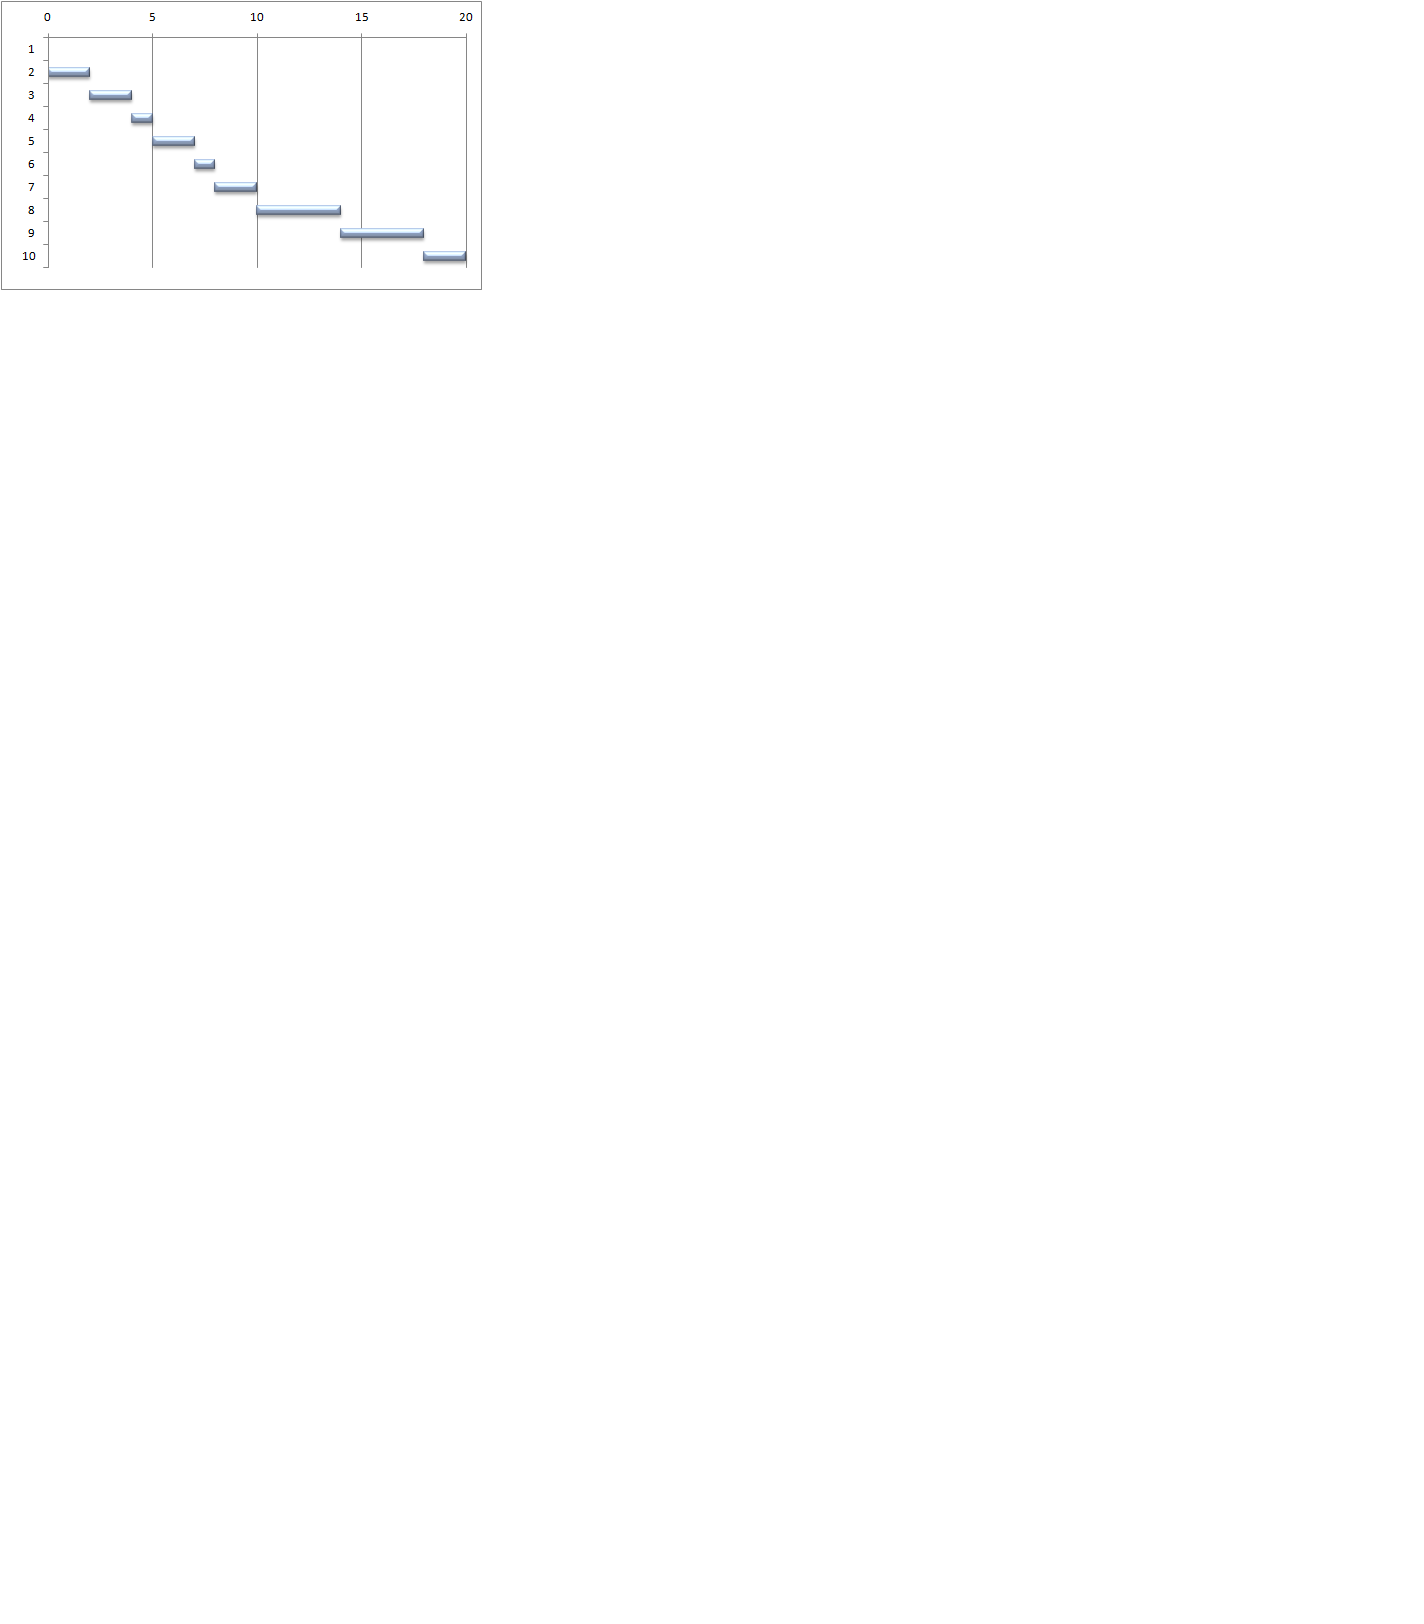
\includegraphics[scale=0.7]{gantt.png}

\begin{thebibliography}{9}

\bibitem{BusinessJavascript}
  W3Techs - World Wide Web Technology Surveys,
  \emph{Usage of JavaScript for websites}.
  \url{http://w3techs.com/technologies/details/cp-javascript/all/all}
  Read on April 9, 2013.

\bibitem{TestingStatistics}
  Mark Bates,
  \emph{Testing Your JavaScript/CoffeeScript}.
  \url{http://www.informit.com/articles/article.aspx?p=1925618}
  Read on April 9, 2013.

\bibitem{GoingFaster}
  Edward Hieatt and Robert Mee,
  \emph{Going Faster: Testing The Web Application}.
  IEEE Software, p.~63
  March/April 2002.

\bibitem{JsUnitGithub}
  Github,
  \emph{pivotal/jsunit}.
  \url{https://github.com/pivotal/jsunit}
  Read on April 3, 2013.

\bibitem{JasmineSite}
  Running documentation,
  \emph{Jasmine is a behavior-driven development framework for testing JavaScript code}.
  \url{http://pivotal.github.com/jasmine/}
  Read on April 3, 2013.

\bibitem{JasmineSpecies}
  Rudy Lattae,
  \emph{Jasmine-species: Extended BDD grammar and reporting for Jasmine}.
  \url{http://rudylattae.github.com/jasmine-species/}
  Read on April 5, 2013.

\bibitem{QUnitSite}
  The jQuery Foundation,
  \emph{QUnit: A JavaScript Unit Testing framework.}
  \url{http://qunitjs.com/}
  Read on April 3, 2013.

\bibitem{MochaSite}
  TJ Holowaychuk,
  \emph{mocha - simple, flexible, fun javascript test framework for node.js \& the browser}.
  \url{http://visionmedia.github.com/mocha/}
  Read on April 3, 2013.

\bibitem{JsTestDriver}
  Cory Smith, Robert Dionne, Vojta Jína, Sergey Simonchik,
  \emph{JsTestDriver}.
  \url{https://code.google.com/p/js-test-driver/}
  Read on April 5, 2013.

\bibitem{BusterJS}
  August Lilleaas, Christian Johansen, et al.,
  \emph{BusterJS: A powerful suite of automated test tools for JavaScript}
  \url{http://docs.busterjs.org/}
  Read on April 5, 2013.

\bibitem{SinonJS}
  Christian Johansen,
  \emph{Sinon.JS: Standalone test spies, stubs and mocks for JavaScript.}
  \url{http://sinonjs.org/}
  Read on April 5, 2013.

\bibitem{Vows}
  Vows: Asynchronous behaviour driven development for Node.
  \url{http://vowsjs.org/}
  Read on April 5, 2013.

\bibitem{Cucumis}
  Cucumis: BDD Cucumber Style Asynchronous Testing Framework for node.js
  \url{https://github.com/noblesamurai/cucumis}
  Read on April 5, 2013.

\bibitem{JSpec}
  JSpec on Github no longer supported
  \url{https://github.com/liblime/jspec}
  Read on April 5, 2013.

\bibitem{AutomatedTesting}
  Shay Artzi, Julian Dolby, Simon Holm Jensen, Anders Møller, Frank Tip,
  \emph{A Framework for Automated Testing of Javascript Web Applications}.
  ICSE ’11, Honolulu, Hawaii, USA.
  May 21–28, 2011.

\bibitem{DOMJavascript}
  Phillip Heidegger, Annette Bieniusa, and Peter Thiemann,
  \emph{DOM Transactions for Testing JavaScript}.
  Albert-Ludwigs-Universität Freiburg, Germany.
  Proceeding TAIC PART'10 Proceedings of the 5th international academic and industrial conference on Testing - practice and research techniques.
  Pages 211-214.
  2010.

\bibitem{Wild}
  Frolin S. Ocariza, Jr., Karthik Pattabiraman, Benjamin Zorn
  \emph{JavaScript Errors in the Wild: An Empirical Study}.
  2011 IEEE 22nd International Symposium on Software Reliability Engineering (ISSRE).
  Pages 100-109.
  Nov. 29 2011-Dec. 2 2011.

\bibitem{Tddjs}
  Christian Johansen,
  \emph{Test-Driven JavaScript Development}
  ADDISON-WESLEY,
  ISBN 9780321683915,
  2010.

\end{thebibliography}

\end{comment}

\section{Draft}

Considering all the different options in available frameworks, one is easily deceived into believing that the main reason why people don't test their JavaScript is because they are lazy or uninformed. This is not necessarily true, there are respectable obstacles for doing TDD both in the process of fitting the frameworks into your application and in writing the JavaScript code in a testable way.

For instance, when setting up JsTestDriver (JSTD) with the Jasmine adapter there are pitfalls in which version you're using. At the time of writing, the latest version of the Jasmine JSTD adapter (1.1) is not compatible with the latest version of Jasmine (1.3.1), so in order to use it you need to find an older version of Jasmine (such as 1.0.1 or 1.1.0) or figure out how to modify the adapter to make it compatible. Moreover, the latest version of JSTD (1.3.5) does not support relative paths to parent folders when referencing script files in jsTestDriver.conf although a few older versions do (such as 1.3.3d), which is a problem if you want to place the test driver separate from the system under test rather than in a parent folder, or if you want to reference another framework such as Jasmine if it is placed in another directory.

Regardless whether or not the frameworks are effortlessly installed and configured or not, there is still the issue of testability. It is common to argue that TDD forces developers to write testable code which tends to be maintainable. This is true in some respects, but one has to bear in mind that JavaScript is commonly used with many side-effects that may not be easily tested. More importantly, it is common to place all the JavaScript code in a single file and hide the implementation using some variant of the module pattern\cite[p.~40]{GoodParts}, which means that only a small subset of the code is exposed as globally accessible functions, commonly functions that are called to initialize some global state such as event listeners. In order to test the functions, they need to be divided into parts, which will typically have to be more general in order to make sense as stand-alone modules. This conflicts with the eagerness of most developers to just get something that works without making it more complicated than necessary.

The fundamental problem is probably that most developers are used to manually test their JavaScript in a browser. This gives an early feedback loop and although it does not come with the benefits of design, quality and automated testing that TDD does, it tends to give a feeling of not doing any extra work and getting the job done as fast as possible. Developers do not want to spend time on mocking dependencies when they are not sure that the solution they have in mind will even work. Once an implementation idea pops up, it can be tempting to just try it out rather than writing tests. If this approach is taken, it may feel like a superfluous task to add tests afterwards since that will typically require some refactoring in order to make the code testable. If the code seems to work good enough, the developer may not be willing to introduce this extra overhead. There is also a risk involved in refactoring untested code\cite[p.~17]{Refactoring}, since manually checking that the refactoring does not introduce bugs is time consuming and difficult to do well, although there is an exception when the refactoring is required in order to add tests. This is because leaving the code untested means even greater risk of bugs and the refactoring may be necessary in the future anyway, in which case it will be even harder and more error-prone.

\nocite{Tddjs}
\printbibliography

\end{document}



